\documentclass[fleqn]{article}

%% Created with wxMaxima 24.11.0

\setlength{\parskip}{\medskipamount}
\setlength{\parindent}{0pt}
\usepackage{iftex}
\ifPDFTeX
  % PDFLaTeX or LaTeX 
  \usepackage[utf8]{inputenc}
  \usepackage[T1]{fontenc}
  \DeclareUnicodeCharacter{00B5}{\ensuremath{\mu}}
\else
  %  XeLaTeX or LuaLaTeX
  \usepackage{fontspec}
\fi
\usepackage{graphicx}
\usepackage{color}
\usepackage[leqno]{amsmath}
\usepackage{ifthen}
\newsavebox{\picturebox}
\newlength{\pictureboxwidth}
\newlength{\pictureboxheight}
\newcommand{\includeimage}[1]{
    \savebox{\picturebox}{\includegraphics{#1}}
    \settoheight{\pictureboxheight}{\usebox{\picturebox}}
    \settowidth{\pictureboxwidth}{\usebox{\picturebox}}
    \ifthenelse{\lengthtest{\pictureboxwidth > .95\linewidth}}
    {
        \includegraphics[width=.95\linewidth,height=.80\textheight,keepaspectratio]{#1}
    }
    {
        \ifthenelse{\lengthtest{\pictureboxheight>.80\textheight}}
        {
            \includegraphics[width=.95\linewidth,height=.80\textheight,keepaspectratio]{#1}
            
        }
        {
            \includegraphics{#1}
        }
    }
}
\newlength{\thislabelwidth}
\DeclareMathOperator{\abs}{abs}

\definecolor{labelcolor}{RGB}{100,0,0}

\begin{document}


\noindent
%%%%%%%%
%% INPUT:
\begin{minipage}[t]{4.000000em}\color{red}\bfseries
(\% i8)	
\end{minipage}
\begin{minipage}[t]{\textwidth}\color{blue}
s:\ t\^\ 4\ -\ 12*t\^\ 3\ +\ 38*t\^\ 2\ -\ 28*t\ +\ 5;
\end{minipage}
%%%% OUTPUT:
\[\displaystyle \tag{s} 
{{t}^{4}}\mathop{-}12 {{t}^{3}}\mathop{+}38 {{t}^{2}}\mathop{-}28 t\mathop{+}5\mbox{}
\]
%%%%%%%%%%%%%%%%


\noindent
%%%%%%%%
%% INPUT:
\begin{minipage}[t]{4.000000em}\color{red}\bfseries
(\% i47)	
\end{minipage}
\begin{minipage}[t]{\textwidth}\color{blue}
wxplot2d([s],[t,0,8],\ [xlabel,"time,\ t(s)"],\ [ylabel,"displacement,\ s(m)"]);
\end{minipage}
%%%% OUTPUT:
\[\displaystyle \tag{\% t47} 
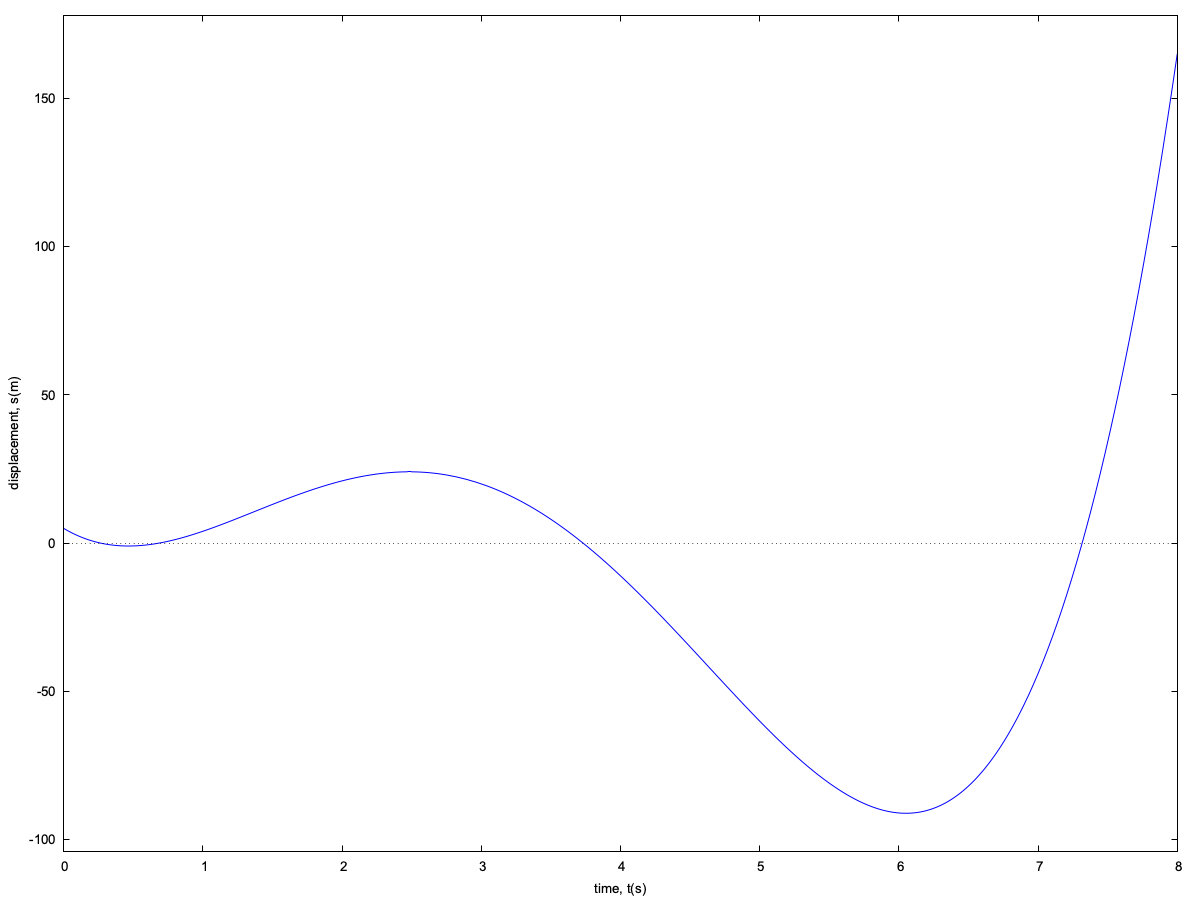
\includegraphics[width=.95\linewidth,height=.80\textheight,keepaspectratio]{question_10_c_img/question_10_c_1}\mbox{}\]

\[\tag{\% o47} 
\mbox{}
\]
%%%%%%%%%%%%%%%%


\noindent
%%%%%%%%
%% INPUT:
\begin{minipage}[t]{4.000000em}\color{red}\bfseries
(\% i31)	
\end{minipage}
\begin{minipage}[t]{\textwidth}\color{blue}
factor(s);
\end{minipage}
%%%% OUTPUT:
\[\displaystyle \tag{\% o31} 
\left( {{t}^{2}}\mathop{-}8 t\mathop{+}5\right) \, \left( {{t}^{2}}\mathop{-}4 t\mathop{+}1\right) \mbox{}
\]
%%%%%%%%%%%%%%%%


\noindent
%%%%%%%%
%% INPUT:
\begin{minipage}[t]{4.000000em}\color{red}\bfseries
(\% i32)	
\end{minipage}
\begin{minipage}[t]{\textwidth}\color{blue}
solve(t\^\ 2-8*t+5,\ t);
\end{minipage}
%%%% OUTPUT:
\[\displaystyle \tag{\% o32} 
\left[ t\mathop{=}4\mathop{-}\sqrt{11}\mathop{,}t\mathop{=}\sqrt{11}\mathop{+}4\right] \mbox{}
\]
%%%%%%%%%%%%%%%%


\noindent
%%%%%%%%
%% INPUT:
\begin{minipage}[t]{4.000000em}\color{red}\bfseries
(\% i33)	
\end{minipage}
\begin{minipage}[t]{\textwidth}\color{blue}
solve(t\^\ 2\ -4*t+1,\ t);
\end{minipage}
%%%% OUTPUT:
\[\displaystyle \tag{\% o33} 
\left[ t\mathop{=}2\mathop{-}\sqrt{3}\mathop{,}t\mathop{=}\sqrt{3}\mathop{+}2\right] \mbox{}
\]
%%%%%%%%%%%%%%%%


\noindent
%%%%%%%%
%% INPUT:
\begin{minipage}[t]{4.000000em}\color{red}\bfseries
(\% i37)	
\end{minipage}
\begin{minipage}[t]{\textwidth}\color{blue}
\\
root1\ :\ 2\ -\ sqrt(3);\\
root2\ :\ 4\ -\ sqrt(11);\\
root3\ :\ 2\ +\ sqrt(3);\\
root4\ :\ 4\ +\ sqrt(11);
\end{minipage}
%%%% OUTPUT:
\[\displaystyle \tag{root1} 
2\mathop{-}\sqrt{3}\mbox{}\]

\[\tag{root2} 
4\mathop{-}\sqrt{11}\mbox{}\]

\[\tag{root3} 
\sqrt{3}\mathop{+}2
\mbox{}\]

\[\tag{root4} 
\sqrt{11}\mathop{+}4\mbox{}
\]
%%%%%%%%%%%%%%%%


\noindent
%%%%%%%%
%% INPUT:
\begin{minipage}[t]{4.000000em}\color{red}\bfseries
(\% i42)	
\end{minipage}
\begin{minipage}[t]{\textwidth}\color{blue}
float(root1);
\end{minipage}
%%%% OUTPUT:
\[\displaystyle \tag{\% o42} 
0.2679491924311228\mbox{}
\]
%%%%%%%%%%%%%%%%
0.27 (to 2 d.p)


\noindent
%%%%%%%%
%% INPUT:
\begin{minipage}[t]{4.000000em}\color{red}\bfseries
(\% i43)	
\end{minipage}
\begin{minipage}[t]{\textwidth}\color{blue}
float(root2);
\end{minipage}
%%%% OUTPUT:
\[\displaystyle \tag{\% o43} 
0.6833752096446002\mbox{}
\]
%%%%%%%%%%%%%%%%
0.68 (to 2 d.p)


\noindent
%%%%%%%%
%% INPUT:
\begin{minipage}[t]{4.000000em}\color{red}\bfseries
(\% i44)	
\end{minipage}
\begin{minipage}[t]{\textwidth}\color{blue}
float(root3);
\end{minipage}
%%%% OUTPUT:
\[\displaystyle \tag{\% o44} 
3.732050807568877\mbox{}
\]
%%%%%%%%%%%%%%%%
3.73 (to 2 d.p)


\noindent
%%%%%%%%
%% INPUT:
\begin{minipage}[t]{4.000000em}\color{red}\bfseries
(\% i45)	
\end{minipage}
\begin{minipage}[t]{\textwidth}\color{blue}
float(root4);
\end{minipage}
%%%% OUTPUT:
\[\displaystyle \tag{\% o45} 
7.3166247903554\mbox{}
\]
%%%%%%%%%%%%%%%%
7.32 (to 2 d.p)
\end{document}
